\chapter{Resultados, Discussões e Trabalhos Futuros}
	\label{capituloFinal}
	
	Em posse da técnica descrita no capítulo \ref{capituloReconstrucao} e dos softwares expostos no capítulo \ref{capituloSoftwares}, foi possível obter resultados com certo grau de corretude e com grande potencial de melhora em sua exatidão.
	
	A seguir são apresentados testes, resultados e discussões acerca das atividades desenvolvidas neste trabalho.
	
	\section{Testes validadores}
		\label{secaoTestes}
		
		Como descrito no capítulo \ref{materiaisEMetodos}, a corretude da técnica desenvolvida, e consequente validade dos resultados obtidos, foi aferida através de cenas específicas (figura \ref{cenasValidacao}) cujos dados foram catalogados previamente.
		
		Após alguns testes preliminares, com valores para a tolerância projetiva igual a $3$ e incremento igual a $0.002$, todas as cenas de validação obtiveram seus mais adequados resultados; dependo, individualmente, apenas do critério arbitrário de convergência.
		
		Para a cena de validação 1 (figura \ref{cenaValidacao1}), cuja montagem de dados está expressa na figura \ref{printTesteCubo}, o melhor critério de convergência foi o de valor de coordenada Z mais próximo ao anteriormente analisado.
		
		Demorando, em média, seis minutos e dez segundos para concluir, a reconstrução da cena de validação 1 retornou os dados da tabela \ref{tabelaErrosCubo}.
		
		\begin{table}
			\caption{Dados da reconstrução da cena de validação 1}
			\label{tabelaErrosCubo}
			\begin{center}
				\begin{tabular}{r r r | r r r | r}
					\hline
					\multicolumn{3}{c}{Obtido} & \multicolumn{3}{c}{Desejado}\\
					\cline{1-6}
					\multicolumn{1}{c}{X} & \multicolumn{1}{c}{Y} & \multicolumn{1}{c}{Z} & \multicolumn{1}{c}{X} & \multicolumn{1}{c}{Y} & \multicolumn{1}{c}{Z} & \multicolumn{1}{c}{Erro geométrico}\\
					\hline			
					0.00625				&			0.007035714		&		0				&		0		&		0		&		0		&		0.009410833\\
					0.996142857		&			0.003428571		&		0				&		1		&		0		&		0		&		0.005160683\\
					0.992					&			0.990393443		&		0				&		1		&		1		&		0		&		0.012501438\\
					0.005571429		& 		0.994571429		&		0				&		0		&		1		&		0		&		0.007778831\\
					0.995111111		&			0.005407407		&		0.99		&		1		&		0		&		1		&		0.012375027\\
					0.997					&			0.998					&		0.99		&		1		&		1		&		1		&		0.010630146\\
					0.010571429		&			0.017492063		&		0.99		&		0		&		0		&		1		&		0.022753624\\
					0.009538462		&			0.995461538		&		0.99		&		0		&		1		&		1		&		0.014545786\\
					\hline
				\end{tabular}
			\end{center}
		\end{table}
		
		Na cena de validação 2 (figura \ref{cenaValidacao2}), cuja montagem de dados é a da figura \ref{printTestePiramide}, o critério de convergência mais eficaz, por sua vez, foi o de valor de coordenada Z mais próximo à média dos valores possíveis.
		
		Com uma demora média para conclusão de quatro minutos, a reconstrução da cena 2 retornou os dados da tabela \ref{tabelaErrosPiramide}.
		
		\begin{table}
			\caption{Dados da reconstrução da cena de validação 2}
			\label{tabelaErrosPiramide}
			\begin{center}
				\begin{tabular}{r r r | r r r | r}
					\hline
					\multicolumn{3}{c}{Obtido} & \multicolumn{3}{c}{Desejado}\\
					\cline{1-6}
					\multicolumn{1}{c}{X} & \multicolumn{1}{c}{Y} & \multicolumn{1}{c}{Z} & \multicolumn{1}{c}{X} & \multicolumn{1}{c}{Y} & \multicolumn{1}{c}{Z} & \multicolumn{1}{c}{Erro geométrico}\\
					\hline			
					0.007					&			0.005					&		0.008		&		0			&		0			&		0		&		0.01174734\\
					0.011866667		&			0.99352				&		0.008		&		0			&		1			&		0		&		0.01571013\\
					0.9675671			&			0.989264069		&		0.008		&		1			&		1			&		0		&		0.035087793\\
					0.982966292		& 		0.004876404		&		0.008		&		1			&		0			&		0		&		0.019440332\\
					0.766722973		&			0.517574324		&		0.904		&		0.5		&		0.5		&		1		&		0.284017607\\
					\hline
				\end{tabular}
			\end{center}
		\end{table}
		
		Na cena de validação 3 (figura \ref{cenaValidacao3}) - montagem da figura \ref{printTesteCuboReduzido}, novamente, o critério de escolher coordenadas Z cujo valor é mais próximo ao plano analisado anteriormente foi o melhor.
		
		Em média, eram gastos seis minutos e vinte segundos para a reconstrução da cena de validação 3 retornar os dados da tabela \ref{tabelaErrosCuboReduzido}.
		
		\begin{table}
			\caption{Dados da reconstrução da cena de validação 3}
			\label{tabelaErrosCuboReduzido}
			\begin{center}
				\begin{tabular}{r r r | r r r | r}
					\hline
					\multicolumn{3}{c}{Obtido} & \multicolumn{3}{c}{Desejado}\\
					\cline{1-6}
					\multicolumn{1}{c}{X} & \multicolumn{1}{c}{Y} & \multicolumn{1}{c}{Z} & \multicolumn{1}{c}{X} & \multicolumn{1}{c}{Y} & \multicolumn{1}{c}{Z} & \multicolumn{1}{c}{Erro geométrico}\\
					\hline			
					0.507521739		&			0.512478261		&		0				&		0.5			&		0.5			&		0			&		0.014569954\\
					0.504075949		&			0.992075949		&		0				&		0.5			&		1				&		0			&		0.008910889\\
					0.989418182		&			0.511109091		&		0				&		1				&		0.5			&		0			&		0.01534232\\
					0.98727027		& 		0.981310811		&		0				&		1				&		1				&		0			&		0.022612647\\
					0.521545455		&			0.521545455		&		0.492		&		0.5			&		0.5			&		0.5		&		0.031502591\\
					0.511					&			0.99575				&		0.492		&		0.5			&		1				&		0.5		&		0.01425\\
					0.9972 				&			0.5164				&		0.492		&		1				&		0.5			&		0.5		&		0.018460769\\
					0.996181818		&			0.995454545		&		0.492		&		1				&		1				&		0.5		&		0.009961911\\
					\hline	
				\end{tabular}
			\end{center}
		\end{table}	
		
		
		
		\begin{figure}[!htb]
			\centering
			\subfloat[Panorama para a reconstrução da cena de validação 1]{
				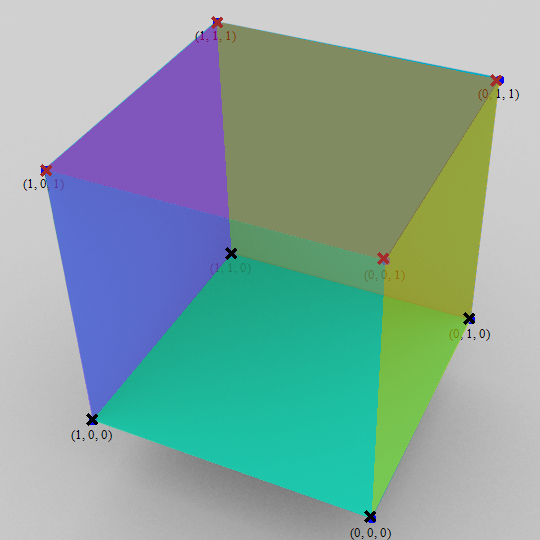
\includegraphics[height=4.5cm]{imagens/printTesteCubo.png}
				\label{printTesteCubo}
			}
			\quad
			\subfloat[Panorama da reconstrução da cena de validação 2]{
				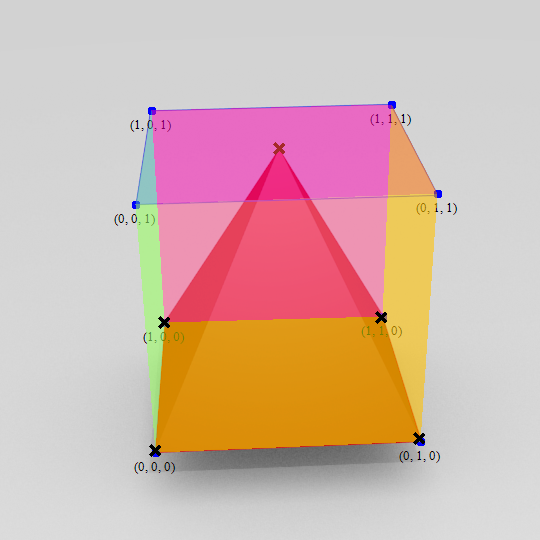
\includegraphics[height=4.5cm]{imagens/printTestePiramide.png}
				\label{printTestePiramide}
			}
			\quad
			\subfloat[Panorama da reconstrução da cena de validação 3]{
				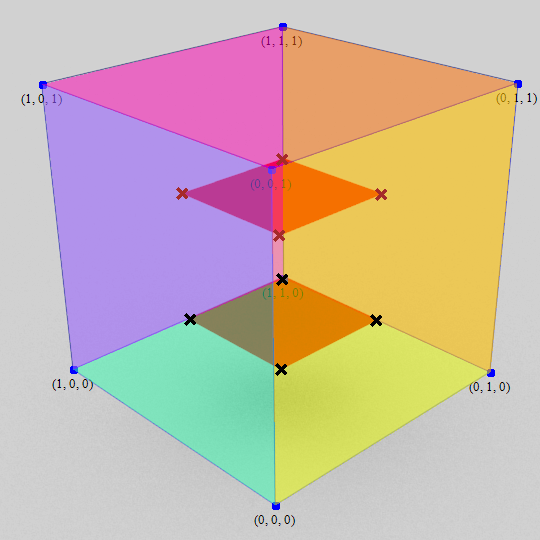
\includegraphics[height=4.5cm]{imagens/printTesteCuboReduzido.png}
				\label{printTesteCuboReduzido}
			}
			\caption{Panoramas das reconstruções de validação}
			\label{printTestes}
		\end{figure}
		
		Através da escolha manual, disponibilizada pelo aplicativo de reconstrução, de valores para as coordenadas Z, há um erro geométrico médio menor entre os pontos, fazendo com que a geometria dos objetos reconstruídos seja mais verossímil. Todavia, a escolha manual é uma estratégia notavelmente brusca e, por isso, resolveu-se não discuti-la nesta monografia.
		
		Todos os dados e resultados dos testes validadores, inclusive os correspondentes à escolha manual, estão disponíveis em \url{https://github.com/ivancezanne/TCC/tree/master/App_Reconstrucao/Testes}.
		
		\section{Resultados}
			\label{secaoResultados}
			
		\section{Discussões}
			\label{secaoDiscussoes}
			
		\section{Trabalhos Futuros}
			\label{secaoTrabalhosFuturos}